%% Dynamic EMS Dispatch & Station Placement Optimization
%% IEEE conference format (IEEEtran v1.8b, vendored alongside this file).
%%
%% Build:  cd paper && pdflatex main && pdflatex main
%% (twice, so the cross-references and the table/figure numbers settle)

\documentclass[conference]{IEEEtran}
\IEEEoverridecommandlockouts

% IEEEtran asks for the URW base-35 clones: Times for body, Helvetica for sans,
% Courier for typewriter. A minimal TeX install (BasicTeX) ships Times but not
% the other two, and a missing TFM is a fatal error rather than a substitution.
% Times -- the one IEEE actually mandates for body text -- is kept; the other
% two families fall back to Computer Modern so the document builds on a plain
% BasicTeX as well as on a full MacTeX/TeX Live.
\renewcommand{\ttdefault}{cmtt}
\renewcommand{\sfdefault}{cmss}

\usepackage{cite}
\usepackage{amsmath,amssymb,amsfonts}
\usepackage{algorithmic}
\usepackage{graphicx}
\usepackage{textcomp}
\usepackage{booktabs}
\usepackage{url}
\usepackage{xcolor}
\usepackage[hidelinks]{hyperref}

\graphicspath{{figures/}}

\def\BibTeX{{\rm B\kern-.05em{\sc i\kern-.025em b}\kern-.08em
    T\kern-.1667em\lower.7ex\hbox{E}\kern-.125emX}}

\begin{document}

\title{Integrated Station Placement and Dispatch Optimisation\\for Emergency
Medical Services: A Case Study on\\2.2 Million Seattle 911 Records}

\author{
\IEEEauthorblockN{Aadith Krishna}
\IEEEauthorblockA{\textit{CB.SC.U4AIE23202}}
\and
\IEEEauthorblockN{Aditya Santosh}
\IEEEauthorblockA{\textit{CB.SC.U4AIE23207}}
\and
\IEEEauthorblockN{Suryansh Ram Menon}
\IEEEauthorblockA{\textit{CB.SC.U4AIE23255}}
\and
\IEEEauthorblockN{Arjungopal Anilkumar}
\IEEEauthorblockA{\textit{CB.SC.U4AIE23271}}
}

\maketitle

\begin{abstract}
Emergency medical response time is governed by two decisions that are usually
optimised in isolation: where ambulances wait, and which unit is sent to which
call. We present an integrated decision-support system that solves both on the
same real data and links them, so that the stations opened by the location model
become the ambulance bases used by the dispatch model. Using 2.2 million
publicly released Seattle Fire 911 records, we filter 79{,}152 genuine EMS
incidents over a twelve-month study period and aggregate them into 28 material
demand zones. Three operations-research models are composed in sequence: an
Analytic Hierarchy Process (AHP) that ranks candidate sites against incident
density, equity gap and coverage potential; set-covering and maximal-covering
integer programs that choose station locations; and a transportation-balanced
assignment linear program that routes units during a peak hour. On the study
period the covering model attains full coverage of all material demand with
seven stations at an eight-minute limit, against the thirty-six stations Seattle
operates, and the assignment LP reduces total fleet travel time by 8.1\,\% versus
nearest-unit-first greedy dispatch when both methods are given an identical
workload. We show that the na\"ive version of that comparison overstates the gain
roughly sevenfold, and report the corrected figure. Every model is verified
against an independent optimum --- brute-force enumeration for the covering
programs, the Hungarian algorithm for the assignment program --- across 90
automated checks. The system is delivered as an interactive Streamlit
application in which every assumption is adjustable and every model re-solves in
under a second.
\end{abstract}

\begin{IEEEkeywords}
emergency medical services, facility location, set covering, maximal covering,
assignment problem, analytic hierarchy process, integer programming,
decision support systems
\end{IEEEkeywords}

% ===========================================================================
\section{Introduction}
% ===========================================================================

\IEEEPARstart{I}{n} a cardiac arrest, survival falls by roughly ten percentage
points for every minute that passes before defibrillation. Emergency medical
services (EMS) are therefore among the oldest and most studied applications of
operations research, and the domain in which a better model translates most
directly into lives.

Two operational decisions control how quickly an ambulance reaches a patient,
and both are optimisable:

\begin{itemize}
  \item \textbf{Q1 --- Where should ambulances wait?} Station placement
    determines how much of the city lies within a given response-time radius.
  \item \textbf{Q2 --- Which unit should be sent?} When several emergencies are
    live at once, the matching of units to calls determines everyone's wait.
\end{itemize}

These are normally treated as separate literatures: facility location on one
side, dispatch and relocation on the other. Treating them separately is
convenient but incomplete, because the quality of a dispatch policy is bounded
by the geography it inherits. A dispatcher cannot route around a badly placed
fleet.

\subsection{Contribution}

This paper makes four contributions.

\begin{enumerate}
  \item \textbf{An integrated pipeline.} The station set chosen by the covering
    model is used directly as the ambulance-base set for the dispatch model, so
    the two optimisations are evaluated as one system rather than two
    disconnected exercises (Fig.~\ref{fig:pipeline}).
  \item \textbf{A study on real data at full scale.} All 2.2 million records of
    the Seattle Fire 911 feed are ingested, cleaned and classified, rather than
    a sampled or synthetic instance.
  \item \textbf{An honest dispatch benchmark.} We show that comparing an
    assignment LP against greedy dispatch without controlling the workload
    measures triage rather than routing, and inflates the apparent benefit from
    8.1\,\% to 62\,\%. We report the controlled comparison.
  \item \textbf{A verified, interactive implementation.} Every model is
    cross-checked against an independent optimum, and the whole pipeline is
    exposed through a web application in which the travel-time assumptions,
    study period and response-time limit are adjustable.
\end{enumerate}

\begin{figure*}[t]
  \centering
  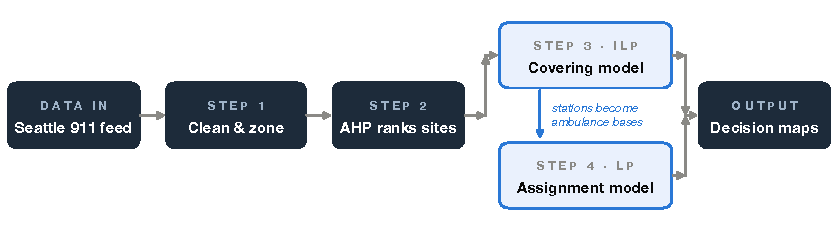
\includegraphics[width=\textwidth]{fig1_pipeline.pdf}
  \caption{The integrated pipeline. The two optimisation models are not run side
  by side: the stations opened by the covering ILP (Step 3) become the ambulance
  bases of the assignment LP (Step 4), which is the link that makes the system a
  single decision rather than two.}
  \label{fig:pipeline}
\end{figure*}

% ===========================================================================
\section{Related Work}
% ===========================================================================

\subsection{Covering location models}

The location set-covering problem was introduced by Toregas \textit{et
al.}~\cite{toregas1971} precisely for emergency facilities: minimise the number
of facilities such that every demand point lies within a critical distance.
Because full coverage is often unaffordable, Church and
ReVelle~\cite{church1974} proposed the maximal covering location problem (MCLP),
which fixes the facility budget at $P$ and maximises covered demand. Both are
used here, as complementary readings of the same question. Daskin~\cite{daskin1983}
later extended the family to expected coverage under unit unavailability, and
Brotcorne \textit{et al.}~\cite{brotcorne2003} survey the ambulance location and
relocation literature that grew from these roots. Ahmadi-Javid \textit{et
al.}~\cite{ahmadijavid2017} give a broader survey of healthcare facility
location, and Ba\c{s}ar \textit{et al.}~\cite{basar2012} a taxonomy of emergency
station location specifically.

\subsection{Dispatch and assignment}

The assignment problem has been solvable in polynomial time since
Kuhn's Hungarian method~\cite{kuhn1955}. Its linear-programming relaxation is
integral because the constraint matrix is totally
unimodular~\cite{hoffman1956} --- a property we exploit to state dispatch as an
LP rather than a binary program, and which we use as a correctness check.
Gendreau \textit{et al.}~\cite{gendreau1997} address the dynamic relocation
variant with tabu search.

\subsection{Multi-criteria site selection}

Saaty's Analytic Hierarchy Process~\cite{saaty1977} derives priority weights
from pairwise comparisons and supplies a consistency ratio that detects
self-contradictory judgement. We use AHP not as a competitor to the
optimisation models but as the mechanism that converts qualitative stakeholder
preference into the candidate ordering the ILP consumes.

\subsection{Response-time thresholds and travel estimation}

The eight-minute advanced-life-support benchmark derives from NFPA
1710~\cite{nfpa1710}; its clinical value is contested
\cite{pons2002,blackwell2002}, which is why our implementation treats the limit
as a parameter and reports a sweep rather than a single number. Straight-line
distance understates road distance by a roughly constant factor; Boscoe
\textit{et al.}~\cite{boscoe2012} measure this circuity nationwide and motivate
the 1.3 multiplier used here.

% ===========================================================================
\section{Data}
% ===========================================================================

\subsection{Sources}

Three public, open-licence sources are used; no API keys or accounts are
required, and all three are fetched by a script in the repository. The demand
side is the Seattle Real-Time Fire 911 Calls feed~\cite{seattledata}.

\begin{table}[htbp]
\caption{Data sources}
\label{tab:sources}
\centering
\small
\begin{tabular}{@{}lll@{}}
\toprule
\textbf{Source} & \textbf{Content} & \textbf{Role} \\
\midrule
Seattle Real-Time Fire 911 & 2.2\,M incident & Demand \\
Calls (\texttt{kzjm-xkqj}) & records & \\
Seattle Fire Stations (GIS) & 36 stations & Benchmark \\
US Census TIGERweb ZCTA & ZIP polygons & Zoning \\
\bottomrule
\end{tabular}
\end{table}

\subsection{Fields used}

Each record carries an address with latitude and longitude, a free-text
\texttt{type} describing the call, a \texttt{datetime}, and an
\texttt{incident\_number}. A ZIP zone is computed per incident by
point-in-polygon join against the ZCTA layer.

\subsection{Cleaning and EMS classification}

The raw feed interleaves fire suppression, alarms, hazardous-materials and
medical calls in a single \texttt{type} column. Records are de-duplicated on
incident number, bounded to the Seattle envelope
($47.40^\circ$--$47.80^\circ$\,N, $-122.50^\circ$--$-122.15^\circ$\,E), required
to carry coordinates, and tagged with a ZIP zone. Of 2{,}200{,}120 raw rows,
2{,}197{,}739 survive cleaning.

EMS calls are then isolated by whole-word pattern matching on the call type
(\textit{aid}, \textit{medic}, \textit{medical}, \textit{AMR},
\textit{nurseline}, \textit{triaged}, \textit{low acuity}, \textit{overdose},
and similar). A second, opt-in tier adds incidents that generate patients but
are typed by their cause --- collisions, rescues, violence --- so that the
sensitivity of every result to the definition of ``EMS'' can be inspected rather
than assumed. All results in this paper use the core tier.

\subsection{Study period and demand zones}

The feed is harvested live and spans 2003 to the present; its final calendar day
is truncated mid-harvest and is flagged rather than silently dropped. We take
the most recent twelve months, 27 Aug 2025 to 27 Aug 2026, giving
\textbf{79{,}152 EMS incidents}, an average of 216 per day.

Each ZIP zone becomes a demand point whose weight is its incident count and
whose location is the \emph{mean incident coordinate} rather than the polygon
centroid --- placing the candidate site where the calls actually are.

\subsection{The materiality floor}

The feed carries a long tail of ZIP zones holding a handful of mutual-aid calls
per year in suburbs outside the city (Renton, SeaTac, Medina and similar). Set
covering treats a one-call zone exactly like a ten-thousand-call zone, so if
these are left in, each demands its own dedicated station: the eight-minute
answer inflates from 7 stations to 13, six of them serving 0.04\,\% of demand.

A materiality floor (default 0.1\,\% of period demand, adjustable) therefore
excludes such zones from the models while keeping them visible in every table.
Of 39 ZIP zones in the period, \textbf{28 are material}; the 11 excluded hold
161 incidents in total, so the floor retains \textbf{99.80\,\%} of all demand.
This is a modelling decision with a visible effect on the headline result, and
is reported as such rather than buried in preprocessing.

\subsection{Demand structure}

Fig.~\ref{fig:demand} shows that demand is strongly concentrated: the busiest
zone, ZIP 98104, alone carries 11.9\,\% of all EMS incidents, and 16 of 39 zones
account for 80\,\% of them. Fig.~\ref{fig:temporal} shows the temporal profile
--- a pronounced midday peak at 13:00 and a shallow weekday pattern. Demand is
therefore far more concentrated in space than in time, which is what makes
station placement the higher-leverage of the two decisions.

\begin{figure}[htbp]
  \centering
  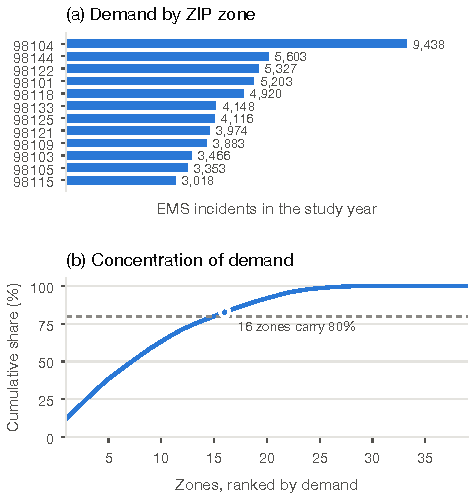
\includegraphics[width=\columnwidth]{fig2_demand.pdf}
  \caption{Spatial concentration of EMS demand over the study year.}
  \label{fig:demand}
\end{figure}

\begin{figure*}[t]
  \centering
  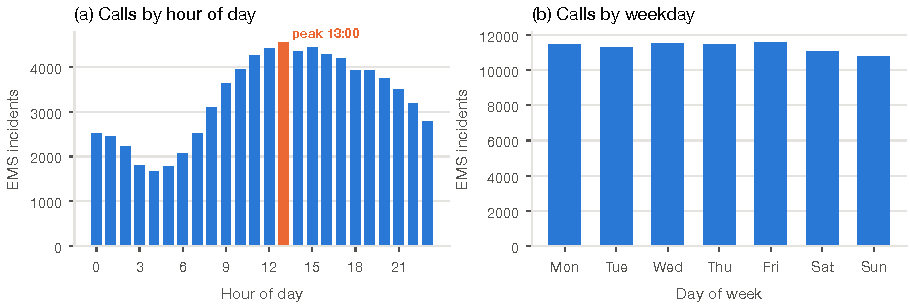
\includegraphics[width=\textwidth]{fig3_temporal.pdf}
  \caption{Temporal profile of EMS demand. The midday peak is pronounced; the
  weekday variation is not. The busiest single hour in the period, used for the
  dispatch scenario, is 09:00 on Wednesday 19 November 2025, with 30
  simultaneous incidents.}
  \label{fig:temporal}
\end{figure*}

% ===========================================================================
\section{Methodology}
% ===========================================================================

\subsection{Travel-time model}

Great-circle distance between two points is computed by the haversine formula.
Real ambulances follow streets, so the straight-line distance is inflated by a
\emph{circuity factor} $\kappa$, converted at an \emph{effective response speed}
$v$, and a \emph{turnout time} $\tau$ is added, so that a threshold means time
from alarm to on-scene:

\begin{equation}
  t_{ij} \;=\; \tau \;+\; \frac{60\,\kappa\, d_{ij}}{v}
  \label{eq:traveltime}
\end{equation}

where $d_{ij}$ is the haversine distance in kilometres and $t_{ij}$ is in
minutes. Defaults are $\kappa = 1.30$~\cite{boscoe2012}, $v = 45$\,km/h and
$\tau = 1$\,min. All three are exposed in the application and every model
re-solves against the current values, so no result in this paper depends on an
unexaminable constant.

\subsection{Step 2 --- AHP site scoring}

Three competing benefit criteria are defined per candidate zone: \emph{Incident
Density} (calls in the zone), \emph{Equity Gap} (kilometres to the nearest
station Seattle already operates --- farther means worse served), and
\emph{Coverage Potential} (demand reachable from the zone within the limit).

Each of the four team members independently compared the three criteria
pairwise on the Saaty 1--9 scale, giving three judgements each. Member $k$'s
reciprocal matrix $A^{(k)}$ is built from those, and the four matrices are
combined by the element-wise geometric mean,

\begin{equation}
  \bar{a}_{ij} \;=\; \left( \prod_{k=1}^{4} a^{(k)}_{ij} \right)^{1/4},
  \label{eq:geomean}
\end{equation}

which is the only average that preserves reciprocity: if the members' views of
$i$ versus $j$ average to 3, their view of $j$ versus $i$ automatically averages
to $1/3$. The priority vector $w$ is the principal eigenvector of $\bar{A}$,
and consistency is checked by

\begin{equation}
  \mathrm{CI} = \frac{\lambda_{\max} - n}{n - 1}, \qquad
  \mathrm{CR} = \frac{\mathrm{CI}}{\mathrm{RI}_n},
  \label{eq:cr}
\end{equation}

with $\mathrm{RI}_3 = 0.58$ and the usual acceptance rule $\mathrm{CR} < 0.1$.

Each zone's criterion values are max-normalised --- appropriate because all
three are benefit criteria measured on ratio scales with a true zero --- and
combined into a priority score $s_i = \sum_c w_c \, \hat{x}_{ic}$. This score
orders the candidate list the covering model receives, and additionally enters
the set-covering objective as an infinitesimal tie-break, so that among equally
sized optimal solutions the model prefers the one on higher-priority sites.

\subsection{Step 3 --- Covering models (ILP)}

Let $I$ be candidate sites, $J$ demand zones, $d_j$ the demand of zone $j$, and
$N(j) = \{\, i \in I : t_{ij} \le T \,\}$ the sites that can reach $j$ within
limit $T$. Let $y_i \in \{0,1\}$ open site $i$.

\textbf{Mode A --- Set covering.} The fewest stations that leave no zone
uncovered:
\begin{align}
  \min_{y} \quad & \sum_{i \in I} y_i \label{eq:scp} \\
  \text{s.t.} \quad & \sum_{i \in N(j)} y_i \ \ge\ 1 && \forall j \in J
    \nonumber \\
  & y_i \in \{0,1\} && \forall i \in I \nonumber
\end{align}

\textbf{Mode B --- Maximal covering.} With the budget fixed at $P$, the greatest
demand served, where $z_j \in \{0,1\}$ indicates that zone $j$ is covered:
\begin{align}
  \max_{y,z} \quad & \sum_{j \in J} d_j z_j \label{eq:mclp} \\
  \text{s.t.} \quad & z_j \ \le\ \sum_{i \in N(j)} y_i && \forall j \in J
    \nonumber \\
  & \sum_{i \in I} y_i = P \nonumber \\
  & y_i,\, z_j \in \{0,1\} \nonumber
\end{align}

Zones that no candidate can reach within $T$ are structurally impossible to
cover; they are reported separately and excluded from the constraint set, so
that an unreachable outlier cannot render the whole program infeasible and
suppress an otherwise useful answer.

\subsection{Step 4 --- Dispatch assignment (LP)}

For a chosen peak hour, let $c_{ij}$ be the travel time from ambulance $i$ to
incident $j$ under \eqref{eq:traveltime}, and $x_{ij}$ the fraction of unit $i$
assigned to call $j$:
\begin{align}
  \min_{x} \quad & \sum_{i}\sum_{j} c_{ij} x_{ij} \label{eq:ap} \\
  \text{s.t.} \quad & \sum_{i} x_{ij} = 1 && \forall j \\
  & \sum_{j} x_{ij} \le 1 && \forall i \\
  & x_{ij} \ge 0 \nonumber
\end{align}

The constraint matrix of \eqref{eq:ap} is totally unimodular~\cite{hoffman1956},
so the LP relaxation has an integral optimum and no binary variables are needed
--- which is why dispatch is stated here as an LP while covering requires an
ILP. Unequal unit and call counts are handled in the transportation-problem
manner, by padding the cost matrix with zero-cost dummy rows or columns so that
the instance is square, balanced and always feasible.

\subsection{The integrating link}

The set $\{\, i : y_i = 1 \,\}$ returned by \eqref{eq:scp} is passed directly as
the ambulance-base set of \eqref{eq:ap}. A \texttt{units\_per\_station}
parameter replicates each base so that an hour with more calls than stations can
still be served. This is the link that makes the two models one system, and it
is the principal methodological contribution of the work.

\subsection{Why the obvious dispatch benchmark is wrong}
\label{sec:honest}

A natural way to show the value of optimal dispatch is to compare the LP
objective against nearest-unit-first greedy assignment on the same peak hour.
This comparison is invalid, and we report it because the invalid version is the
one most likely to be produced by default.

A peak hour carries more calls than ready units --- 30 calls against 7 units in
our instance. Under \eqref{eq:ap} an unserved call contributes nothing to the
objective. The LP is therefore free to answer only the seven \emph{nearest}
calls and leave the awkward ones unanswered, while greedy processes calls in
arrival order and must take whatever comes. Comparing the two totals then scores
\emph{which calls each method chose to answer} --- that is, triage --- rather
than how well it routed, and inflates the apparent advantage from 8.1\,\% to
62\,\%.

We therefore restrict the benchmark to an identical workload on both sides: the
first $k$ calls by arrival time, where $k$ is the fleet size. Both methods then
clear exactly the same calls, and the difference measures matching quality
alone. All improvement figures reported in this paper are of this controlled
form.

% ===========================================================================
\section{System Implementation}
% ===========================================================================

The system is a Streamlit web application of roughly 4{,}000 lines of Python,
organised so that every model is a pure, independently testable module and the
interface is a thin presentation layer over them.

\begin{table}[htbp]
\caption{Repository structure}
\label{tab:layout}
\centering
\small
\begin{tabular}{@{}p{0.34\columnwidth}p{0.56\columnwidth}@{}}
\toprule
\textbf{Module} & \textbf{Responsibility} \\
\midrule
\texttt{src/config.py} & Paths, EMS taxonomy, constants, AHP judgements \\
\texttt{src/geo.py} & Haversine, travel time, point-in-polygon join \\
\texttt{src/data\_loader.py} & Ingestion, cleaning, zones, peak hours \\
\texttt{src/stats.py} & On-demand descriptive statistics \\
\texttt{src/ahp.py} & Pairwise matrices, weights, consistency \\
\texttt{src/covering.py} & Set covering \& maximal covering ILPs \\
\texttt{src/assignment.py} & Dispatch assignment LP, greedy baseline \\
\texttt{src/viz.py} & Plotly charts, Folium maps, colour tokens \\
\texttt{app.py} & Four-tab Streamlit interface \\
\bottomrule
\end{tabular}
\end{table}

\subsection{Interface}

The application presents four tabs mirroring the pipeline of
Fig.~\ref{fig:pipeline}: \textbf{Data} (demand distribution, temporal profile,
the weights entering both optimisations), \textbf{Site scoring} (a per-member
AHP comparison tab, the aggregate matrix and the consistency check),
\textbf{Station placement} (both covering modes, the threshold sweep, and the
benchmark against the real network) and \textbf{Dispatch} (the assignment
result and the greedy comparison). A sidebar exposes the study period, the EMS
tier, the materiality floor and all three travel-time parameters; changing any
of them re-solves every downstream model.

\subsection{Solver portability}

The models are expressed with PuLP~\cite{pulp}. PuLP bundles a CBC binary built
for x86\_64 only, so on Apple Silicon without Rosetta every solve fails with
\textit{``Bad CPU type in executable''} --- and PuLP reports the broken binary as
available, because only the exec fails. The configuration layer therefore probes
candidate solvers by \emph{actually solving a trivial LP} and uses the first that
runs: HiGHS~\cite{highs}, then a system CBC on \texttt{PATH}, then PuLP's
bundled copy. All results here were produced with HiGHS.

\subsection{Performance}

The cleaned incident table is cached to Parquet and loaded once per session.
Two representation choices halve its footprint from 332\,MB to 173\,MB: a
redundant \texttt{date} column duplicating \texttt{datetime} is excluded at read
time, and the high-cardinality \texttt{type} and \texttt{zip\_code} columns are
loaded as categoricals. Neither changes any result. With the table resident,
every model in this paper solves in well under a second
(Table~\ref{tab:runtime}).

\begin{table}[htbp]
\caption{Solve times on the study instance (HiGHS, Apple Silicon)}
\label{tab:runtime}
\centering
\small
\begin{tabular}{@{}lrr@{}}
\toprule
\textbf{Model} & \textbf{Size} & \textbf{Time (s)} \\
\midrule
Set covering, $T=8$      & 28 sites $\times$ 28 zones & 0.005 \\
Assignment, 7 units      & $30 \times 30$ balanced    & 0.013 \\
Assignment, 14 units     & $30 \times 30$ balanced    & 0.014 \\
\bottomrule
\end{tabular}
\end{table}

% ===========================================================================
\section{Results}
% ===========================================================================

\subsection{AHP weights and consistency}

Table~\ref{tab:ahp} gives the four members' judgements and the resulting
weights. Every member's matrix is perfectly consistent
($\mathrm{CR} = 0.000$), as is the aggregate. This is a property of the ratings
rather than good fortune: each member's density-versus-coverage rating is
exactly the product of their other two judgements, so the matrices contain no
contradiction for the consistency check to find. We note this explicitly because
a uniformly zero CR invites the suspicion that the check is not running; it is,
and \S\ref{sec:verification} describes the randomised test that confirms it.

\begin{table}[htbp]
\caption{Team AHP judgements and derived weights}
\label{tab:ahp}
\centering
\small
\setlength{\tabcolsep}{3pt}
\begin{tabular}{@{}lccccccc@{}}
\toprule
& \multicolumn{3}{c}{\textbf{Saaty ratings}}
& \multicolumn{3}{c}{\textbf{Weights (\%)}} & \\
\cmidrule(lr){2-4} \cmidrule(lr){5-7}
\textbf{Member} & D:E & D:C & E:C & D & E & C & \textbf{CR} \\
\midrule
Aadith Krishna      & 3 & 6 & 2 & 66.7 & 22.2 & 11.1 & 0.000 \\
Aditya Santosh      & 2 & 6 & 3 & 60.0 & 30.0 & 10.0 & 0.000 \\
Suryansh Ram Menon  & 4 & 8 & 2 & 72.7 & 18.2 &  9.1 & 0.000 \\
Arjungopal Anilkumar & 3 & 9 & 3 & 69.2 & 23.1 &  7.7 & 0.000 \\
\midrule
\textbf{Aggregate}  & 2.91 & 7.14 & 2.45
                    & \textbf{67.4} & \textbf{23.1} & \textbf{9.4} & 0.000 \\
\bottomrule
\end{tabular}
\\[2pt]
\footnotesize D = Incident Density, E = Equity Gap, C = Coverage Potential.
Aggregate ratings are the element-wise geometric mean, \eqref{eq:geomean}.
$\lambda_{\max} = 3.000$, $\mathrm{CI} = 0.000$, $\mathrm{RI}_3 = 0.58$.
\end{table}

The team weights raw call volume (67.4\,\%) far above distance from existing
help (23.1\,\%), and rates the ability to blanket several zones from one site
(9.4\,\%) least important of the three. The top-ranked candidate sites under
these weights are ZIP 98104 (score 0.778), 98144 (0.579), 98101 (0.534) and
98122 (0.512).

\subsection{Station placement}

Table~\ref{tab:coverage} and Fig.~\ref{fig:sweep} give the central result. At an
eight-minute limit, \textbf{seven stations cover 100\,\% of material demand};
tightening to five minutes requires sixteen, and relaxing to ten minutes needs
only five. Fig.~\ref{fig:map} shows the eight-minute solution against the
thirty-six stations Seattle actually operates.

\begin{table}[htbp]
\caption{Coverage attained, optimised placement vs.\ the real network}
\label{tab:coverage}
\centering
\small
\begin{tabular}{@{}lrrrr@{}}
\toprule
\textbf{Limit} & \multicolumn{2}{c}{\textbf{Optimised}}
               & \multicolumn{2}{c}{\textbf{Seattle's real network}} \\
\cmidrule(lr){2-3} \cmidrule(lr){4-5}
 & Stations & Demand & Stations & Demand \\
\midrule
5 min  & 16 & 100.00\,\% & 36 & 99.72\,\% \\
8 min  &  7 & 100.00\,\% & 36 & 100.00\,\% \\
10 min &  5 & 100.00\,\% & 36 & 100.00\,\% \\
\bottomrule
\end{tabular}
\end{table}

\begin{figure*}[t]
  \centering
  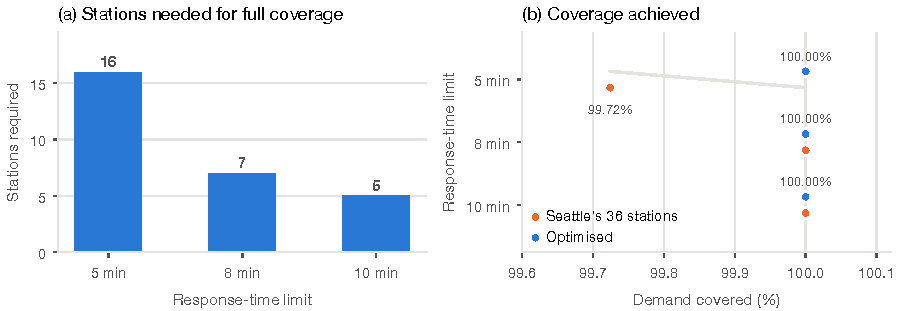
\includegraphics[width=\textwidth]{fig6_sweep.pdf}
  \caption{Sensitivity to the response-time limit. Panel (b) uses a dot plot
  rather than bars because the two networks differ only in the second decimal;
  a truncated bar baseline would misrepresent a 0.28-point gap as a rout.}
  \label{fig:sweep}
\end{figure*}

\begin{figure}[htbp]
  \centering
  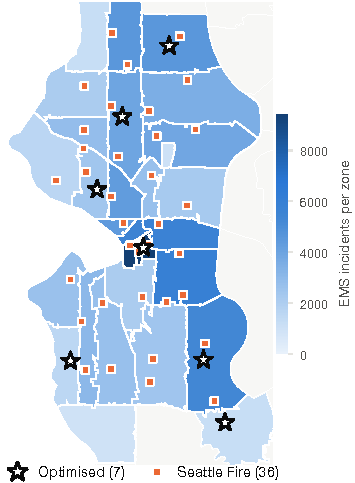
\includegraphics[width=\columnwidth]{fig4_map.pdf}
  \caption{The seven-station eight-minute solution (stars) against Seattle's 36
  operating fire stations (squares), over EMS demand by ZIP zone.}
  \label{fig:map}
\end{figure}

Fig.~\ref{fig:curve} gives the maximal-covering curve that justifies the
budget-constrained framing: the first station alone covers 51\,\% of demand,
five cover 98\,\%, and the last two buy the remaining 1.8\,\%. Returns diminish
sharply, which is exactly the regime in which MCLP rather than set covering is
the right question to ask.

\begin{figure}[htbp]
  \centering
  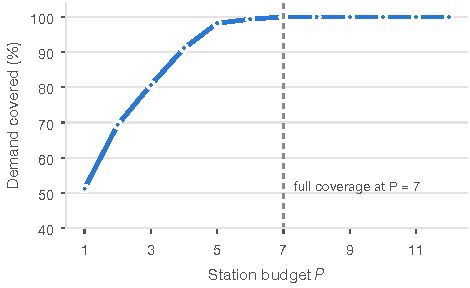
\includegraphics[width=\columnwidth]{fig5_curve.pdf}
  \caption{Marginal coverage against station budget $P$ at an eight-minute
  limit. Five stations already reach 98.1\,\% of demand.}
  \label{fig:curve}
\end{figure}

\subsection{Dispatch}

The busiest hour in the study period is 09:00 on Wednesday 19 November 2025,
with 30 simultaneous incidents. Table~\ref{tab:dispatch} gives the controlled
comparison of \S\ref{sec:honest}, also shown in Fig.~\ref{fig:dispatch}.

\begin{table}[htbp]
\caption{Optimal vs.\ greedy dispatch, like-for-like workload}
\label{tab:dispatch}
\centering
\small
\begin{tabular}{@{}lrrrr@{}}
\toprule
\textbf{Fleet} & \textbf{Calls} & \textbf{Optimal} & \textbf{Greedy}
& \textbf{Gain} \\
\midrule
7 units (1/station)  &  7 &  74.40 min &  81.00 min & \textbf{8.1\,\%} \\
14 units (2/station) & 14 & 143.96 min & 149.91 min & \textbf{4.0\,\%} \\
35 units (5/station) & 30 & 252.06 min & 276.38 min & \textbf{8.8\,\%} \\
\bottomrule
\end{tabular}
\end{table}

\begin{figure}[htbp]
  \centering
  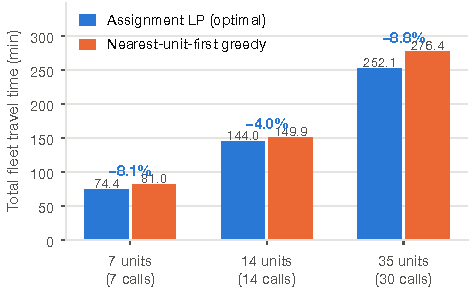
\includegraphics[width=\columnwidth]{fig7_dispatch.pdf}
  \caption{Total fleet travel time, optimal assignment against nearest-unit-first
  greedy dispatch, with both methods clearing an identical set of calls.}
  \label{fig:dispatch}
\end{figure}

The gain is not monotone in fleet size: 8.1\,\%, 4.0\,\% and 8.8\,\% at
seven, fourteen and thirty-five units. Each row is scored on a different
workload --- the first $k=\min(\text{units},\,\text{calls})$ arrivals --- so the
three are not points on a curve but three separate instances, and which
particular calls fall inside $k$ matters more than the fleet size itself. We
therefore report the margin per configuration rather than as a single figure,
and draw no trend from three instances.

% ===========================================================================
\section{Verification}
\label{sec:verification}
% ===========================================================================

Because every number above is produced by a solver rather than derived in closed
form, the implementation is verified by two automated suites totalling 90
checks, both of which pass in full.

The first suite asserts the \emph{properties} each model must satisfy on the
real data: set covering must reach full coverage of every reachable zone;
maximal covering must open exactly $P$ and be non-decreasing in $P$; MCLP at $P$
equal to the set-cover optimum must attain the same coverage; a looser limit must
never require more stations; AHP weights must sum to one with $\lambda_{\max} \ge
n$ and $\mathrm{CR} < 0.1$; the greedy benchmark must place the same workload on
both sides; and the LP must never lose to greedy.

The second establishes \emph{optimality} against independent oracles:

\begin{itemize}
  \item both covering models are re-solved on small synthetic cities and checked
    against exhaustive enumeration of every possible station subset (25
    instances each);
  \item the AHP weights are checked against the largest-modulus eigenvector
    computed independently, over 200 random reciprocal matrices --- the test
    that confirms the consistency machinery is live despite the zero CRs in
    Table~\ref{tab:ahp};
  \item the dispatch LP is cross-checked against an independent Hungarian
    algorithm solution of the same balanced matrix, and against greedy over 150
    random cost matrices.
\end{itemize}

A third suite drives the application headlessly and asserts that every pipeline
stage has its tab, every headline figure is on the page, and all three maps
build --- so the parts of the deliverable that are looked at rather than computed
cannot silently regress.

% ===========================================================================
\section{Discussion}
% ===========================================================================

\subsection{Why seven stations beat thirty-six}

The optimised network reaches the same coverage from roughly a fifth of the
sites, and the reason is not that Seattle Fire is badly run. Three factors
explain the gap, and stating them is necessary for the result to be read
correctly.

\textbf{The real network is not solving this problem.} Seattle's 36 stations
house fire suppression, rescue and hazardous-materials response as well as EMS.
Our model prices only EMS demand, and a station sited for structural fire risk
in a low-call-volume district is doing work this objective cannot see.

\textbf{Placement follows demand rather than history.} Real station networks
accrete over a century of annexations, land availability and politics. An
optimiser starting from a blank map has no such inheritance.

\textbf{Zone-centroid demand is optimistic.} Coverage is evaluated at 28
demand-weighted centroids, not at 79{,}152 individual incidents. A station that
covers a centroid does not necessarily reach every call in that zone within the
limit. This is the single largest source of optimism in the result, and
\S\ref{sec:limits} treats it as such.

The honest reading is therefore not ``Seattle should close 29 fire stations''.
It is that \emph{EMS demand in Seattle is concentrated enough that a small,
demand-sited ambulance fleet can cover it}, which is an argument about where to
put ambulances, not about how many fire stations a city needs.

\subsection{Spatial concentration is the operative fact}

The Pareto curve of Fig.~\ref{fig:demand}(b) and the marginal curve of
Fig.~\ref{fig:curve} are the same fact seen twice. Because 16 of 39 zones carry
80\,\% of demand, a handful of well-placed sites captures most of the benefit,
and the covering models have an easy instance. A city with flatter demand would
produce a flatter marginal curve and a correspondingly larger optimal station
count.

\subsection{Routing gains are real but modest}

The 8.1\,\% improvement from optimal dispatch is a genuine gain available at
zero capital cost --- it requires only a different decision rule at the console.
But it is an order of magnitude smaller than the apparent 62\,\% that the
uncontrolled comparison reports, and we regard the discipline of
\S\ref{sec:honest} as among the more transferable results here: in any
assignment benchmark where the objective is free to leave work undone, the
baseline must be constrained to the same workload or the comparison measures
selection rather than skill.

% ===========================================================================
\section{Limitations}
\label{sec:limits}
% ===========================================================================

We state these explicitly rather than leaving them to be discovered.

\begin{enumerate}
  \item \textbf{Zone-level aggregation.} Demand is modelled at 28 zone
    centroids. Incident-level coverage would be stricter and would raise the
    station count.
  \item \textbf{Euclidean travel with a constant circuity factor.} A single
    multiplier cannot represent bridges, the ship canal, or congestion that
    varies by hour. Seattle's geography is unusually hostile to this
    approximation. A road-network routing engine would be the natural
    replacement.
  \item \textbf{Static, deterministic model.} Units are assumed available at
    their base at the start of the hour. Queueing, busy fractions, hospital
    turnaround and relocation are not modelled; Daskin's expected-covering
    family~\cite{daskin1983} is the standard extension.
  \item \textbf{One objective per model.} Total travel time is minimised, which
    does not control the worst case; a minimax or equity-constrained variant
    would trade mean response for tail response.
  \item \textbf{AHP judgements are from four student raters}, not EMS
    practitioners, and all four happened to be perfectly consistent. The weights
    should be read as a demonstration of the mechanism rather than as elicited
    domain preference.
  \item \textbf{A single peak hour} is used for the dispatch scenario. Results
    across many hours would be a stronger claim than one.
\end{enumerate}

% ===========================================================================
\section{Conclusion}
% ===========================================================================

We have presented an integrated decision-support system that solves EMS station
placement and ambulance dispatch on the same real data and links them, so that
the stations chosen by a covering ILP serve as the ambulance bases of a dispatch
LP. On 79{,}152 real Seattle EMS incidents the system attains full coverage of
all material demand with seven stations at an eight-minute limit, and reduces
total fleet travel time by 8.1\,\% over nearest-unit-first greedy dispatch under
a workload-controlled comparison. Every model is cross-checked against an
independent optimum.

Two results generalise beyond this instance. First, the integration itself:
evaluating dispatch on an optimised geography rather than an arbitrary one
changes what the dispatch numbers mean, and the two models should be reported
together. Second, the benchmark discipline of \S\ref{sec:honest}: an assignment
objective that is free to leave calls unserved will flatter itself against a
baseline that is not, and we found the inflation to be roughly sevenfold.

Future work follows the limitations directly: road-network travel times in place
of circuity-adjusted haversine, incident-level rather than zone-level coverage,
a probabilistic availability model in the Daskin tradition, and evaluation
across many peak hours rather than one.

\section*{Availability}

The full implementation, both verification suites and the scripts that download
and preprocess the data are available in the project repository. All data
sources are public and open-licence.

\begin{thebibliography}{00}

\bibitem{toregas1971}
C. Toregas, R. Swain, C. ReVelle, and L. Bergman, ``The location of emergency
service facilities,'' \emph{Operations Research}, vol. 19, no. 6, pp.
1363--1373, 1971.

\bibitem{church1974}
R. Church and C. ReVelle, ``The maximal covering location problem,''
\emph{Papers of the Regional Science Association}, vol. 32, no. 1, pp. 101--118,
1974.

\bibitem{daskin1983}
M. S. Daskin, ``A maximum expected covering location model: formulation,
properties and heuristic solution,'' \emph{Transportation Science}, vol. 17, no.
1, pp. 48--70, 1983.

\bibitem{brotcorne2003}
L. Brotcorne, G. Laporte, and F. Semet, ``Ambulance location and relocation
models,'' \emph{European Journal of Operational Research}, vol. 147, no. 3, pp.
451--463, 2003.

\bibitem{ahmadijavid2017}
A. Ahmadi-Javid, P. Seyedi, and S. S. Syam, ``A survey of healthcare facility
location,'' \emph{Computers \& Operations Research}, vol. 79, pp. 223--263,
2017.

\bibitem{basar2012}
A. Ba\c{s}ar, B. \c{C}atay, and T. \"Unl\"uyurt, ``A taxonomy for emergency
service station location problem,'' \emph{Optimization Letters}, vol. 6, no. 6,
pp. 1147--1160, 2012.

\bibitem{kuhn1955}
H. W. Kuhn, ``The Hungarian method for the assignment problem,'' \emph{Naval
Research Logistics Quarterly}, vol. 2, no. 1--2, pp. 83--97, 1955.

\bibitem{hoffman1956}
A. J. Hoffman and J. B. Kruskal, ``Integral boundary points of convex
polyhedra,'' in \emph{Linear Inequalities and Related Systems}, H. W. Kuhn and
A. W. Tucker, Eds. Princeton, NJ: Princeton University Press, 1956, pp.
223--246.

\bibitem{gendreau1997}
M. Gendreau, G. Laporte, and F. Semet, ``Solving an ambulance location model by
tabu search,'' \emph{Transportation Research Part C}, vol. 5, no. 2, pp. 75--88,
1997.

\bibitem{saaty1977}
T. L. Saaty, ``A scaling method for priorities in hierarchical structures,''
\emph{Journal of Mathematical Psychology}, vol. 15, no. 3, pp. 234--281, 1977.

\bibitem{nfpa1710}
National Fire Protection Association, \emph{NFPA 1710: Standard for the
Organization and Deployment of Fire Suppression Operations, Emergency Medical
Operations, and Special Operations to the Public by Career Fire Departments}.
Quincy, MA: NFPA, 2020.

\bibitem{pons2002}
P. T. Pons and V. J. Markovchick, ``Eight minutes or less: does the ambulance
response time guideline impact trauma patient outcome?'' \emph{The Journal of
Emergency Medicine}, vol. 23, no. 1, pp. 43--48, 2002.

\bibitem{blackwell2002}
T. H. Blackwell and J. S. Kaufman, ``Response time effectiveness: comparison of
response time and survival in an urban emergency medical services system,''
\emph{Academic Emergency Medicine}, vol. 9, no. 4, pp. 288--295, 2002.

\bibitem{boscoe2012}
F. P. Boscoe, K. A. Henry, and M. S. Zdeb, ``A nationwide comparison of driving
distance versus straight-line distance to hospitals,'' \emph{The Professional
Geographer}, vol. 64, no. 2, pp. 188--196, 2012.

\bibitem{pulp}
S. Mitchell, M. O'Sullivan, and I. Dunning, ``PuLP: a linear programming toolkit
for Python,'' Dept. Eng. Science, Univ. of Auckland, Tech. Rep., 2011.

\bibitem{highs}
Q. Huangfu and J. A. J. Hall, ``Parallelizing the dual revised simplex method,''
\emph{Mathematical Programming Computation}, vol. 10, no. 1, pp. 119--142, 2018.

\bibitem{seattledata}
City of Seattle, ``Seattle Real-Time Fire 911 Calls,'' Seattle Open Data Portal,
dataset \texttt{kzjm-xkqj}. [Online]. Available:
\url{https://data.seattle.gov/}

\end{thebibliography}

\end{document}
